% LaTeX Template For MATH 490 @ VCU
\documentclass{article}

\usepackage{graphicx}
\usepackage{hyperref}
\usepackage{amsmath}
\usepackage{amsthm}
\usepackage{amssymb}
\usepackage{verbatim}

\graphicspath{{../plot/}}

\begin{document}


\title{Lab 1 - Vector and Matrix Operations\\
\large{Numerical Methods in Physics}}
\author{Kamil Śmigielski}

\maketitle

\section{Introduction}

The aim of this laboratory class was to implement basic vector operations using C++17, investigate the convergence or divergence of select matrix raised to given power, and compare calculation efficiency of single thread matrix multiplication with CBLAS matrix multiplication.

\section{Method}

The select matrix was defined as:

\begin{equation}
    A_{i,j} = \frac{1}{|i-j|^4 + \gamma},(\gamma =2, 3),(i,j=0,1,2,...,n-1)
\end{equation}
Where the given vector was defined as:
\begin{equation}
    x_{i} = 1,(i=0,1,2,...,n-1)
\end{equation}
The matrix A and vector x was represented as a continous C++ vector of double type variables to accomodate for precision. The main process then calculates the product of vector and matrix, and records the reported norm.

To compare calculation performance on two-dimensional arrays, two programs with the sole purpouse of exponentiating a large matrix A 30 times were prepared, and their runtimes. Two seperate methods of calculation were used, single thread algorithm, and imported CBLAS cblas\_dgemm method.
Matrix multiplication is defined as:
\begin{equation}
    AA:= A_{i,k} =\sum_{j = 1}^{n-1}A_{i,j}*B_{j,k}  
\end{equation}
For my implementation, i implemented a fucnction matrix\_times\_vec with the following code:
\newpage 
\begin{verbatim}
void matrix_times_vec(const std::vector<double>* A, std::vector<double>* x){
  std::vector<double> x_new(LDA, 0.0);
  for(int j=0; j<LDA; j++){
    double sum = 0.0;
    for(int i=0; i<LDA; i++){
      sum += (*x)[i] * (*A)[i + j*LDA];
    };
    x_new[j] = sum;
  };
  *x = x_new;
}
\end{verbatim}

\section{Analysis}

\begin{center}
    \centering
    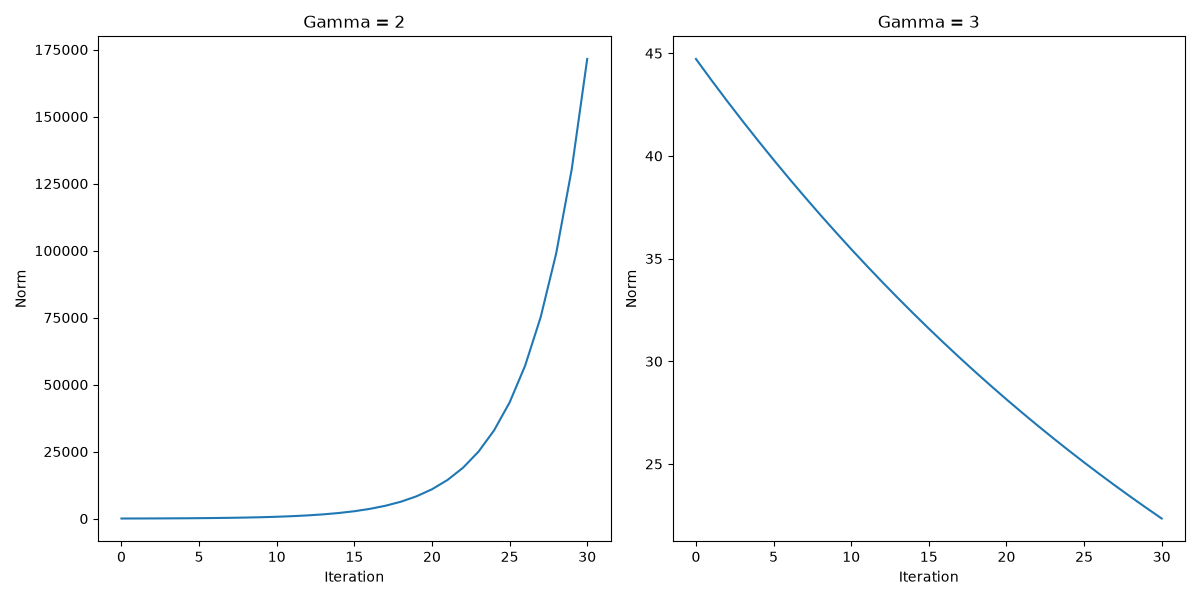
\includegraphics[width=\textwidth]{plot.png}
    \small{Figure 1: Presented are two plots for differing gamma values}
\end{center}
For two differing gamma values, we see differing behaviour. For gamma values differing by a mere value of 1, the vector norm's converge/diverge.

\begin{table}[h]
\centering
\begin{tabular}{|c|c|c|}
\hline
             & Pure C++ & CBLAS implementation \\
\hline
$\gamma = 2$ & 20.8258s                     & 0.190630s             \\
$\gamma = 3$ & 20.7631s                     & 0.162376s            \\ \hline
\end{tabular}
\caption{Runtime comparison between single-thread and CBLAS implementations.}
\end{table}

The program runtime was sped up by a factor of $10^3$, which is an undeniable improvement. This difference in execution speed will only grow with matrix input, and it's calculations process dosen't seem to not contain any disatvantages.

\section{Conclusion}
Our given matrix $A$ convergant behaviour is prone to high fluxuations based on given $\gamma$ parameter.\\
The CBLAS library computes matrix multiplication significantly faster than naive, close to definition algorithm implementations of matrix multiplication.
\end{document}